% Options for packages loaded elsewhere
\PassOptionsToPackage{unicode}{hyperref}
\PassOptionsToPackage{hyphens}{url}
%
\documentclass[
  ignorenonframetext,
]{beamer}
\usepackage{pgfpages}
\setbeamertemplate{caption}[numbered]
\setbeamertemplate{caption label separator}{: }
\setbeamercolor{caption name}{fg=normal text.fg}
\beamertemplatenavigationsymbolsempty
% Prevent slide breaks in the middle of a paragraph
\widowpenalties 1 10000
\raggedbottom
\setbeamertemplate{part page}{
  \centering
  \begin{beamercolorbox}[sep=16pt,center]{part title}
    \usebeamerfont{part title}\insertpart\par
  \end{beamercolorbox}
}
\setbeamertemplate{section page}{
  \centering
  \begin{beamercolorbox}[sep=12pt,center]{part title}
    \usebeamerfont{section title}\insertsection\par
  \end{beamercolorbox}
}
\setbeamertemplate{subsection page}{
  \centering
  \begin{beamercolorbox}[sep=8pt,center]{part title}
    \usebeamerfont{subsection title}\insertsubsection\par
  \end{beamercolorbox}
}
\AtBeginPart{
  \frame{\partpage}
}
\AtBeginSection{
  \ifbibliography
  \else
    \frame{\sectionpage}
  \fi
}
\AtBeginSubsection{
  \frame{\subsectionpage}
}

\usepackage{amsmath,amssymb}
\usepackage{iftex}
\ifPDFTeX
  \usepackage[T1]{fontenc}
  \usepackage[utf8]{inputenc}
  \usepackage{textcomp} % provide euro and other symbols
\else % if luatex or xetex
  \usepackage{unicode-math}
  \defaultfontfeatures{Scale=MatchLowercase}
  \defaultfontfeatures[\rmfamily]{Ligatures=TeX,Scale=1}
\fi
\usepackage{lmodern}
\ifPDFTeX\else  
    % xetex/luatex font selection
\fi
% Use upquote if available, for straight quotes in verbatim environments
\IfFileExists{upquote.sty}{\usepackage{upquote}}{}
\IfFileExists{microtype.sty}{% use microtype if available
  \usepackage[]{microtype}
  \UseMicrotypeSet[protrusion]{basicmath} % disable protrusion for tt fonts
}{}
\makeatletter
\@ifundefined{KOMAClassName}{% if non-KOMA class
  \IfFileExists{parskip.sty}{%
    \usepackage{parskip}
  }{% else
    \setlength{\parindent}{0pt}
    \setlength{\parskip}{6pt plus 2pt minus 1pt}}
}{% if KOMA class
  \KOMAoptions{parskip=half}}
\makeatother
\usepackage{xcolor}
\newif\ifbibliography
\setlength{\emergencystretch}{3em} % prevent overfull lines
\setcounter{secnumdepth}{-\maxdimen} % remove section numbering


\providecommand{\tightlist}{%
  \setlength{\itemsep}{0pt}\setlength{\parskip}{0pt}}\usepackage{longtable,booktabs,array}
\usepackage{calc} % for calculating minipage widths
\usepackage{caption}
% Make caption package work with longtable
\makeatletter
\def\fnum@table{\tablename~\thetable}
\makeatother
\usepackage{graphicx}
\makeatletter
\def\maxwidth{\ifdim\Gin@nat@width>\linewidth\linewidth\else\Gin@nat@width\fi}
\def\maxheight{\ifdim\Gin@nat@height>\textheight\textheight\else\Gin@nat@height\fi}
\makeatother
% Scale images if necessary, so that they will not overflow the page
% margins by default, and it is still possible to overwrite the defaults
% using explicit options in \includegraphics[width, height, ...]{}
\setkeys{Gin}{width=\maxwidth,height=\maxheight,keepaspectratio}
% Set default figure placement to htbp
\makeatletter
\def\fps@figure{htbp}
\makeatother

\makeatletter
\@ifpackageloaded{caption}{}{\usepackage{caption}}
\AtBeginDocument{%
\ifdefined\contentsname
  \renewcommand*\contentsname{Table of contents}
\else
  \newcommand\contentsname{Table of contents}
\fi
\ifdefined\listfigurename
  \renewcommand*\listfigurename{List of Figures}
\else
  \newcommand\listfigurename{List of Figures}
\fi
\ifdefined\listtablename
  \renewcommand*\listtablename{List of Tables}
\else
  \newcommand\listtablename{List of Tables}
\fi
\ifdefined\figurename
  \renewcommand*\figurename{Figure}
\else
  \newcommand\figurename{Figure}
\fi
\ifdefined\tablename
  \renewcommand*\tablename{Table}
\else
  \newcommand\tablename{Table}
\fi
}
\@ifpackageloaded{float}{}{\usepackage{float}}
\floatstyle{ruled}
\@ifundefined{c@chapter}{\newfloat{codelisting}{h}{lop}}{\newfloat{codelisting}{h}{lop}[chapter]}
\floatname{codelisting}{Listing}
\newcommand*\listoflistings{\listof{codelisting}{List of Listings}}
\makeatother
\makeatletter
\makeatother
\makeatletter
\@ifpackageloaded{caption}{}{\usepackage{caption}}
\@ifpackageloaded{subcaption}{}{\usepackage{subcaption}}
\makeatother
\ifLuaTeX
  \usepackage{selnolig}  % disable illegal ligatures
\fi
\usepackage{bookmark}

\IfFileExists{xurl.sty}{\usepackage{xurl}}{} % add URL line breaks if available
\urlstyle{same} % disable monospaced font for URLs
\hypersetup{
  pdftitle={Reviewing the exchange rate},
  pdfauthor={I Made Krisna Gupta},
  hidelinks,
  pdfcreator={LaTeX via pandoc}}

\title{Reviewing the exchange rate}
\subtitle{ECEU603002 Keuangan internasional}
\author{I Made Krisna Gupta}
\date{September 5, 2024}

\begin{document}
\frame{\titlepage}

\begin{frame}{Reminder}
\phantomsection\label{reminder}
\begin{itemize}
\item
  Your lecturer pre-midterm is I Made Krisna aka
  \href{https://krisna.or.id}{Imed}.

  \begin{itemize}
  \tightlist
  \item
    contents are mostly to catch you up with trade theories.
  \end{itemize}
\item
  Kiki Verico will handle post-midterm.
\item
  As discussed, we will use contents from Feenstra \& Taylor's
  International Macroeconomics.

  \begin{itemize}
  \tightlist
  \item
    pictures, graphs, tables with no explicit source is from the book.
  \end{itemize}
\item
  Slides, homeworks, and announcements will be on EMAS (at least
  pre-midterm).
\end{itemize}
\end{frame}

\begin{frame}{Eploring questions}
\phantomsection\label{eploring-questions}
\begin{enumerate}
\tightlist
\item
  Fitur apa dari nilai tukar yang perlu kita perhatikan?
\item
  Bagaimana operasionalisasi pasar uang?
\item
  ekspektasi dan arbitrasi penting. KOk bisa?
\end{enumerate}
\end{frame}

\begin{frame}{Pendahuluan}
\phantomsection\label{pendahuluan}
\begin{itemize}
\item
  Nilai tukar sangat berpengaruh pada perdagangan internasional barang
  dan jasa, tapi juga jual beli aset keuangan.
\item
  Dampak ini datang lewat harga barang dan jasa, serta harga aset
  (bonds, stocks, harga rumah dan lain lain)
\item
  Perdagangan di pasar uang bernilai triliunan dolar dan terkadang
  memiliki implikasi yang sangat besar.
\end{itemize}
\end{frame}

\begin{frame}{Topik hari ini}
\phantomsection\label{topik-hari-ini}
\begin{itemize}
\item
  Dasar dari nilai tukar
\item
  Fakta tentang pergerangan nilai tukar
\item
  Pasar uang
\item
  Arbitrase dan ekspektasi
\end{itemize}
\end{frame}

\begin{frame}{Dasar nilai tukar}
\phantomsection\label{dasar-nilai-tukar}
\begin{itemize}
\item
  Nilai tukar (E) adalah harga satu mata uang yang
  diekspresikan/dinilai/divaluasi dalam mata uang lain.
\item
  Karena nilai tukar pada dasarnya adalah harga relatif, maka E dapat
  diekspresikan dengan dua cara:

  \begin{itemize}
  \item
    Rupiah yang diperlukan untuk membeli 1 unit mata uang lain; atau
  \item
    Mata uang lain yang diperlukan untuk membeli 1 unit rupiah.
  \end{itemize}
\item
  Biasanya kami jelaskan mana yang menjadi \emph{home country} dan mana
  yang jadi \emph{foreign country}.
\item
  Misalnya ketika kita bicara tentang Indonesia sebagai \emph{home
  country}, maka nilai tukar Indonesia akan diekspresikan sebagai rupiah
  yang diperlukan untuk 1 dolar AS.
\end{itemize}
\end{frame}

\begin{frame}{Harga IDR}
\phantomsection\label{harga-idr}
\begin{longtable}[]{@{}llll@{}}
\caption{Nilai tukar Rupiah
(\href{https://www.bi.go.id/id/statistik/ekonomi-keuangan/seki/Default.aspx\#headingFour}{Tabel
V.40 SEKI})}\tabularnewline
\toprule\noalign{}
Jenis Valuta & May-24 & Jun-24 & Jul-24 \\
\midrule\noalign{}
\endfirsthead
\toprule\noalign{}
Jenis Valuta & May-24 & Jun-24 & Jul-24 \\
\midrule\noalign{}
\endhead
USD & 16.253 & 16.421 & \emph{16.320} \\
EUR & 17.569 & 17.554 & 17.655 \\
GBP & 20.656 & 20.746 & 20.972 \\
SGD & 12.023 & 12.096 & 12.144 \\
JPY/100 & 10.353 & 10.228 & 10.540 \\
\bottomrule\noalign{}
\end{longtable}

\(E_{\$/Rp}=6,127\times 10^{-5}\) U.S. exchange rate (America terms)

\(E_{Rp/\$}=16.320\) Indonesian exchange rate (Indo terms)

\(E_{Rp/\$,t}=\frac{1}{E_{\$/Rp,t}}\)
\end{frame}

\begin{frame}{Apredepre}
\phantomsection\label{apredepre}
\begin{itemize}
\item
  Jika 1 Rp dapat membeli lebih banyak dolar, kita katakan Rp
  \emph{menguat}, \emph{naik harga}, atau \emph{apresiasi} terhadap
  dolar.
\item
  Jika 1 Rp dapat membeli lebih sedikit dolar, kita katakan Rp
  \emph{melemah}, \emph{turun harga}, atau \emph{depresiasi} terhadap
  dolar.
\item
  Jika Rupiah menguat terhadap Dolar, maka Dolar melemah terhadap
  Rupiah.
\item
  Karena kita biasa menulis nilai tukar rupiah sebagai \(E_{Rp/\$}\),
  maka angkanya jadi kebalik. Angkanya naik = depresiasi.
\item
  Apresiasi dan depresiasi biasanya diekspresikan dalam persen, atau
  \(\frac{\Delta E_{t}}{E_t}=\frac{E_{t+1}-E_{t}}{E_{t}}\)
\end{itemize}
\end{frame}

\begin{frame}{Apredepre}
\phantomsection\label{apredepre-1}
\begin{longtable}[]{@{}lll@{}}
\toprule\noalign{}
Jenis Valuta & Jul-23 & Jul-24 \\
\midrule\noalign{}
\endhead
IDR/USD & 15.083 & \emph{16.320} \\
USD/IDR & 6.63e-05 & \emph{6.127e-05} \\
\bottomrule\noalign{}
\end{longtable}

Perubahan nilai rupiah tahunan di bulan Juli jadinya adalah:

\[
\frac{\Delta E_{\$/Rp}}{E_{\$/Rp}}=\frac{16320-15083}{15083}=0,082=8,2\%
\]

Rupiah terdepresiasi 8,2\% terhadap dolar.
\end{frame}

\begin{frame}{Apredepre}
\phantomsection\label{apredepre-2}
\begin{longtable}[]{@{}lll@{}}
\toprule\noalign{}
Jenis Valuta & Jul-23 & Jul-24 \\
\midrule\noalign{}
\endhead
IDR/USD & 15.083 & \emph{16.320} \\
USD/IDR & 6.63e-05 & \emph{6.127e-05} \\
\bottomrule\noalign{}
\end{longtable}

Perubahan nilai dolar adalah:

\[
\frac{\Delta E_{Rp/\$}}{E_{Rp/\$}}=\frac{6,127-6,63}{6,63}=-0,0759=-7,59\%
\]

Dolar terapresiasi 7,59\% terhadap rupiah.
\end{frame}

\begin{frame}{Multilateral XR}
\phantomsection\label{multilateral-xr}
\begin{itemize}
\item
  Dihitung dengan melakukan agregasi nilai tukar bilateral dengan
  menggunakan bobot berdasarkan nilai perdagangan.
\item
  Hasilnya disebut juga dengan \emph{effective exchange rate}.
\item
  Misalnya 40\% perdagangan Home adalah dengan negara 1 dan 60\% dengan
  negara 2. Nilai tukar Home apresiasi 10\% terhadap 1 tapi depresiasi
  30\% terhadap 2.
\item
  Nilai tukar efektif Home adalah:
\end{itemize}

(−10\% • 40\%) + (30\% • 60\%) = (−0.1 • 0.4) + (0.3 • 0.6) = −0.04 +
0.18 = 0.14 = +14\%.

Home's effective exchange rate terdepresiasi 14\%.
\end{frame}

\begin{frame}{Perbandingan harga}
\phantomsection\label{perbandingan-harga}
\begin{figure}[H]

{\centering 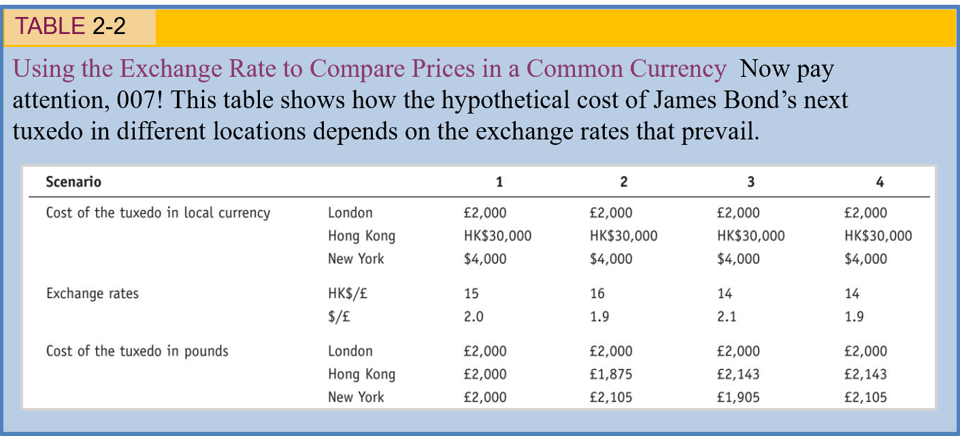
\includegraphics{Picture1.png}

}

\caption{Di mana James Bond harus membeli tuxedonya?}

\end{figure}%
\end{frame}

\begin{frame}{Rezim nilai tukar}
\phantomsection\label{rezim-nilai-tukar}
2 jenis rezim nilai tukar utama adalah:

\begin{itemize}
\item
  Fixed (pegged) exchange rate: nilai tukar cenderung stabil atau sangat
  kecil volatilitasnya terhadap \emph{base currecny}. Agar ini bisa
  tercapai, pemerintah / bank sentral harus intervensi (gak gratis).
\item
  Floating (flexible) exchange rate: nilai tukar berfluktuasi lebih
  lebar dibanding pegged. Pasar uang berpengaruh lebih tinggi dan
  intervensi pemerintah sangat minimal. Perubahan bisa terjadi tiap
  detik.
\end{itemize}
\end{frame}

\begin{frame}{Contoh rezim XR}
\phantomsection\label{contoh-rezim-xr}
\begin{figure}[H]

{\centering 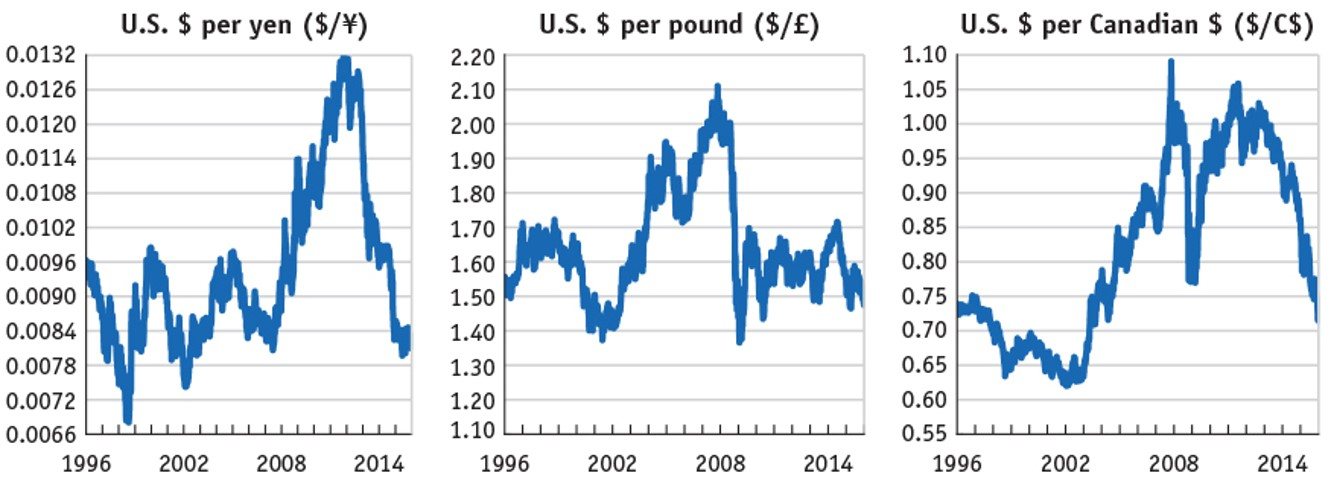
\includegraphics{Picture2.jpg}

}

\caption{Ini adalah nilai tukar dolar AS terhadap 3 nilai tukar utama.
Nilai tukar dolar AS cenderung volatil karena AS menerapkan free float
rezim.}

\end{figure}%
\end{frame}

\begin{frame}{Contoh rezim XR}
\phantomsection\label{contoh-rezim-xr-1}
\begin{figure}[H]

{\centering 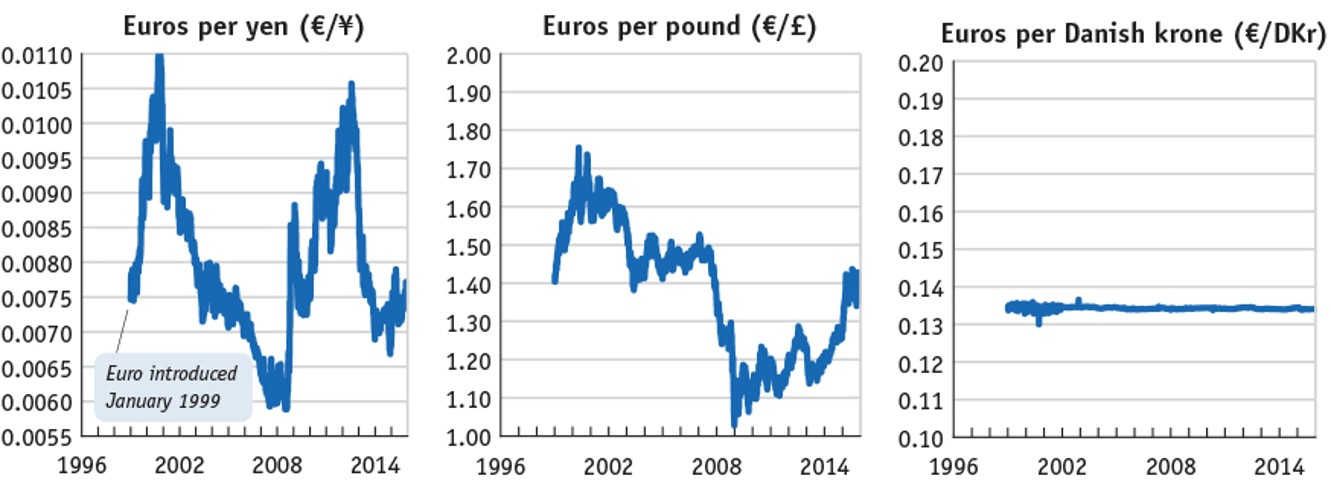
\includegraphics{Picture3.jpg}

}

\caption{Ini adalah nilai tukar 3 mata uang terhadap Euro. Yen dan pound
float terhadap euro. Krone menerapkan fixed exchange rate dengan
toleransi 2\% perubahan terhadap euro (disebut juga band).}

\end{figure}%
\end{frame}

\begin{frame}{Contoh rezim XR}
\phantomsection\label{contoh-rezim-xr-2}
\begin{figure}[H]

{\centering 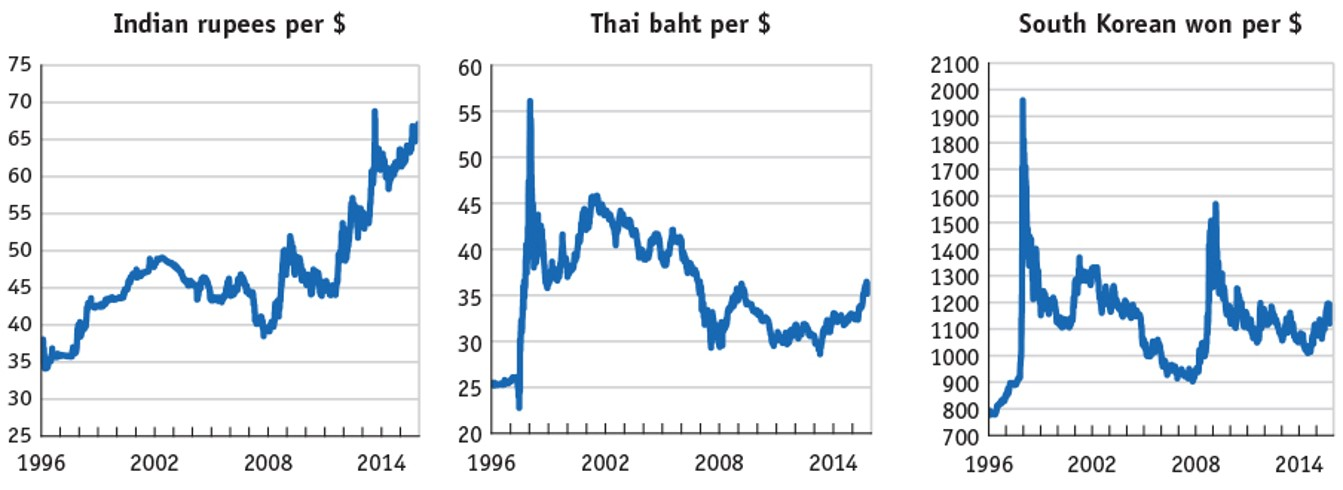
\includegraphics{Picture4.jpg}

}

\caption{Nilai tukar di negara berkembang menunjukkan volatilitas yang
agak terbatas (biasanya dipeg terbatas atau managed float), tapi juga
dampak periode krisis yang sangat terlihat.}

\end{figure}%
\end{frame}

\begin{frame}{Contoh rezim XR}
\phantomsection\label{contoh-rezim-xr-3}
\begin{figure}[H]

{\centering 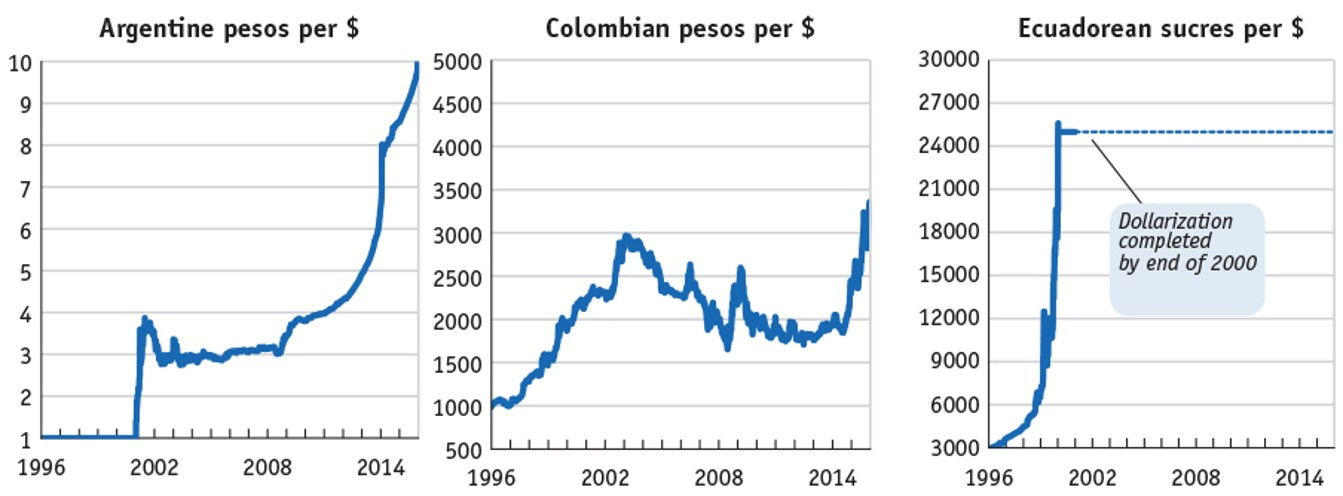
\includegraphics{Picture5.jpg}

}

\caption{Kolombia adalah contoh crawling peg, di mana peg dilakukan dan
depresiasi dilakukan pelan-pelan. Sementara itu Ekuador melakukan
dolarisasi,di mana mata uang mereka sepenuhnya tergantung pada AS}

\end{figure}%
\end{frame}

\begin{frame}{XR Indonesia}
\phantomsection\label{xr-indonesia}
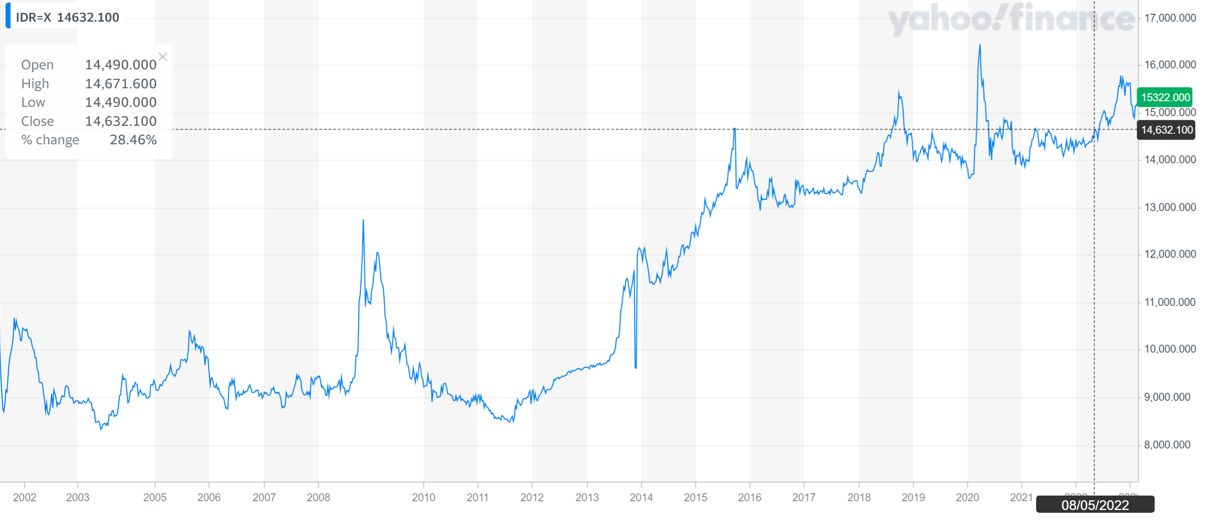
\includegraphics{idr2.png}

Indonesia memiliki nilai tukar yang ada di tengah, atau managed
floating. Tidak begitu ketat, tapi juga tidak terbang bebas. Bisa
dikatakan kita melakukan managed float. Data ini didapat dari
\href{https://yhoo.it/3ZaTko7}{Yahoo finance}.
\end{frame}

\begin{frame}{Rezim XR}
\phantomsection\label{rezim-xr}
\begin{figure}[H]

{\centering 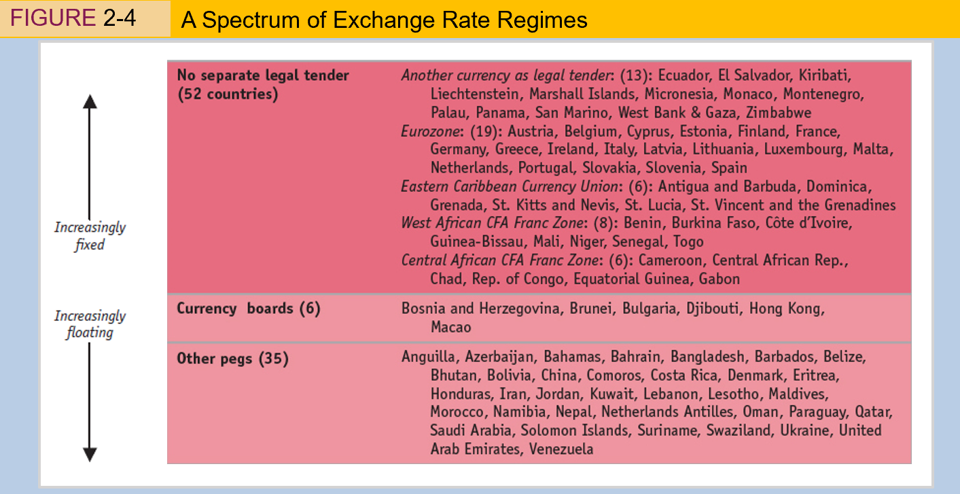
\includegraphics{regime.png}

}

\caption{Gambar ini didapat oleh Feenstra Taylor dari IMF, yang
melakukan klasifikasi terhadap 182 negara. Rezim XR merupakan spektrum
dari yang paling fix sampai paling float. 6 negara melakukan ultrapeg
yang namanya currency board.}

\end{figure}%
\end{frame}

\begin{frame}{Pasar uang}
\phantomsection\label{pasar-uang}
\begin{itemize}
\item
  nilai tukar diatur di pasar uang, atau pasar forex atau \emph{foreign
  exchange market} atau FX Market.
\item
  Dibilang ``diatur'' juga sebenarnya tidak ada 1 institusi yang
  mengatur. Pasar ini adalah pasar terdesentralisasi yang terdiri dari
  bank, perusahaan, pemerintah, dan investor.
\item
  In January 2013, the global forex market traded \$5.3 trillion per day
  in currency.
\item
  Pasar uang paling ramai saat ini ada di London, New York, Tokyo,
  Singapura, dan Hong Kong.
\end{itemize}
\end{frame}

\begin{frame}{Spot contract}
\phantomsection\label{spot-contract}
\begin{itemize}
\item
  Transaksi paling simpel adalah kontrak ``on the spot'' atau nilai yang
  langsung diberikan. Disebut juga \emph{spot contract}.
\item
  Exchange rate yang digunakan disebut juga \emph{spot price} atau
  \emph{spot exchange rate} atau \emph{spot rate}.
\item
  Nilai spot rate inilah yang biasanya muncul di berita-berita dan
  secara umum.
\item
  Spot contract adalah metode yang paling umum, sebanyak 90\% total
  transaksi nilai tukar.
\end{itemize}
\end{frame}

\begin{frame}{Derivatives}
\phantomsection\label{derivatives}
\begin{itemize}
\item
  Selain spot, perdagangan mata uang juga dilakukan dengan kontrak lain,
  yaitu forwards, swaps, futures dan options.
\item
  Secara kolektif, keempat kontrak ini disebut dengan derivatives.
\item
  Spot rate dan forward rate biasanya tidak begitu berbeda.
\end{itemize}
\end{frame}

\begin{frame}{Derivatives}
\phantomsection\label{derivatives-1}
\begin{itemize}
\item
  Forward contract dilakukan hari ini, dengan harga hari ini, tapi
  pembayaran (settlement) dilakukan di masa depan (settlement date).
  Karena itu dapat dikatakan forward contract tidak ada risikonya.
\item
  Kontrak swap adalah kombinasi spot dan forward, di mana kontrak
  dieksekusi saat itu juga (seperti spot) dengan perjanjian repurchase
  atau pembelian kembali di masa depan (seperti forward). Kombinasi 2
  transaksi ini dapat menurunkan biaya transaksi.
\end{itemize}
\end{frame}

\begin{frame}{Derivatives}
\phantomsection\label{derivatives-2}
\begin{itemize}
\item
  Kontrak future adalah perjanjian pertukaran valas di masa depan dengan
  harga yang sudah ditentukan, seperti halnya forward. Bedanya dengan
  forward, kontrak ini terstandar, mature-nya juga di tanggal yang
  standar, dan dapat diperdagangkan di bursa.
\item
  Options memberikan izin pada pembeli untuk membeli (call) atau menjual
  (put) valas di masa depan dengan harga yang sudah ditentukan. Pembeli
  options tidak harus tunduk pada kontrak tersebut jika spot rate
  ternyata lebih baik.
\end{itemize}
\end{frame}

\begin{frame}{Manfaat derivatives}
\phantomsection\label{manfaat-derivatives}
\begin{itemize}
\item
  Derivatives berguna untuk mengurangi risiko nilai tukar. atau malah
  berspekulasi terhadap nilai tukar.
\item
  Example 1: Hedging. As chief financial officer of a U.S. firm, you
  expect to receive payment of €1 million in 90 days for exports to
  France. The current spot rate is \$1.20 per euro. Your firm will incur
  losses on the deal if the euro weakens to less than \$1.10 per euro.
  You advise that the firm buy €1 million in call options on dollars at
  a rate of \$1.15 per euro, ensuring that the firm's euro receipts will
  sell for at least this rate. This locks in a minimal profit even if
  the spot rate falls below \$1.15. This is hedging.
\end{itemize}
\end{frame}

\begin{frame}{Manfaat derivatives}
\phantomsection\label{manfaat-derivatives-1}
\begin{itemize}
\item
  Derivatives berguna untuk mengurangi risiko nilai tukar. atau malah
  berspekulasi terhadap nilai tukar.
\item
  Example 2: Speculation. The market currently prices one-year euro
  futures at \$1.30, but you think the dollar will weaken to \$1.43 in
  the next 12 months. If you wish to make a bet, you would buy these
  futures, and if you are proved right, you will realize a 10\% profit.
  Any level above \$1.30 will generate a profit. If the dollar is at or
  below \$1.30 a year from now, however, your investment in futures will
  be a total loss. This is speculation.
\end{itemize}
\end{frame}

\begin{frame}{Aktor pasar uang}
\phantomsection\label{aktor-pasar-uang}
\begin{itemize}
\item
  Bank komersil merupakan aktor paling sering melakukan perdagangan
  forex. 75\% transaksi forex dieksekusi oleh hanya 10 bank.
\item
  Nilai tukar yang sering dijadikan acuan adalah hasil aktivitas mereka.
\item
  Perusahaan non-bank bisa saja berdagang di pasar uang langsung jika
  banyak menggunakan valas.
\item
  Pemerintah dapat melakukan intervensi dengan merestriksi perdagangan
  forex atau transaksi finansial antar-negara. Intervensi ini disebut
  \emph{capital control}.
\item
  Akibatnya Bank sentral akan jadi lebih aktif di pasar uang.
\end{itemize}
\end{frame}

\begin{frame}{Arbitrase}
\phantomsection\label{arbitrase}
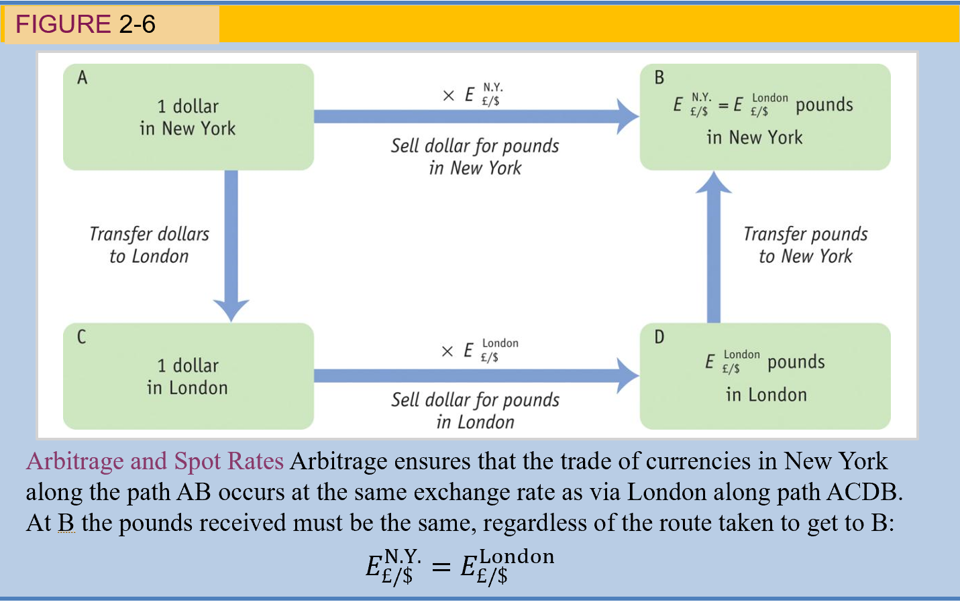
\includegraphics{Picture6.png}
\end{frame}

\begin{frame}{Arbitrase}
\phantomsection\label{arbitrase-1}
3 kemungkinan dalam arbitrase 3 mata uang.

\begin{enumerate}
\tightlist
\item
  Direct trade lebih menguntungkan, atau \(E_{£/\$}>E_{£/€}E_{€/\$}\).
\item
  Indirect trade lebih menguntungkan, atau \(E_{£/\$}<E_{£/€}E_{€/\$}\).
\item
  Tidak ada yang lebih menguntungkan, atau \(E_{£/\$}=E_{£/€}E_{€/\$}\).
  Di sini, tidak ada peluang untuk arbitrase. Disebut juga
  \emph{no-arbitrage condition}.
\end{enumerate}
\end{frame}

\begin{frame}{Arbitrase}
\phantomsection\label{arbitrase-2}
\[
\underbrace{E_{£/\$}}_{\text{direct exchange rate}}=E_{£/€}E_{€/\$}=\underbrace{\frac{E_{£/€}}{E_{\$/€}}}_{\text{cross  rate}}
\]

Rasio dari 2 exchange rate disebut juga dengan \emph{cross rate}.
Prinsipnya sama dengan \emph{chain rule} dalam kalkulus.
\end{frame}

\begin{frame}{Arbitrase}
\phantomsection\label{arbitrase-3}
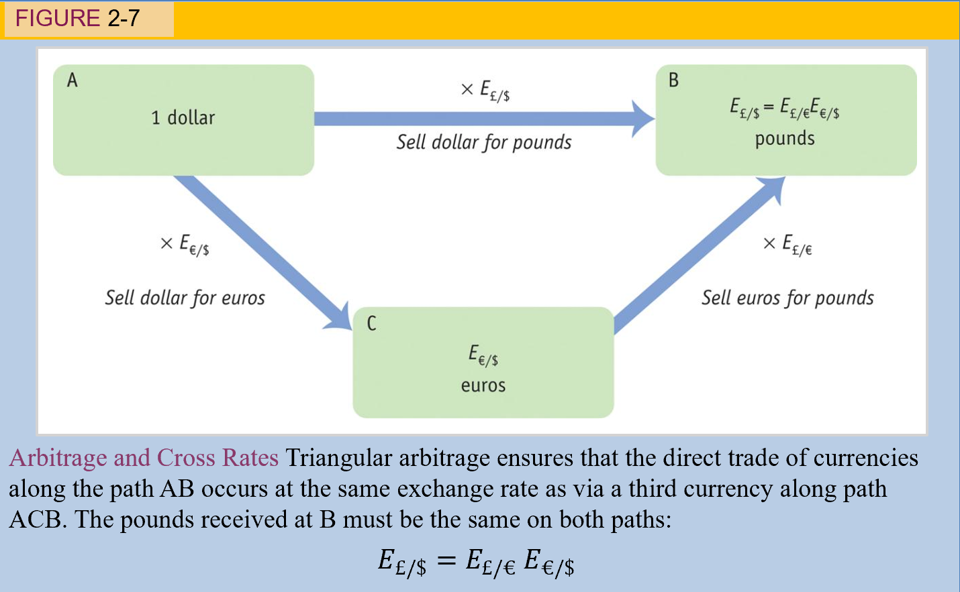
\includegraphics{Picture7.png}
\end{frame}

\begin{frame}{Arbitrase}
\phantomsection\label{arbitrase-4}
\begin{itemize}
\item
  Mayoritas valas dunia diperdagangankan secara langsung hanya dengan
  satu atau dua valas utama seperti dolar AS, yen, euro, dan pound.
\item
  Banyak negara melakukan bisnis internasional dalam dolar AS atau valas
  utama lain, sehingga seseorang selalu dapat menggunakan dolar AS untuk
  \emph{triangular trade}.
\item
  Ketika 2 negara berdagang dengan menggunakan mata uang negara ke-3,
  mata uang tersebut dinamakan \emph{vehicle currency}, karena mata uang
  tersebut hanya menjadi perantara.
\end{itemize}
\end{frame}

\begin{frame}{Arbitrase dan return}
\phantomsection\label{arbitrase-dan-return}
\begin{itemize}
\item
  Pertanyaan penting bagi investor adalah dalam mata uang apa seorang
  investor menyimpan asetnya?
\item
  Seandainya saya punya rupiah nganggur, apakah sebaiknya dibiarkan atau
  diconvert ke dolar?
\item
  Keputusan ini akan mempengaruhi permintaan mata uang relatif serta
  menentukan nilai tukarnya.
\item
  Beli bond rupiah = dapat return rupiah, tapi beli bond dolar = beli
  dolar sekarang -\textgreater{} beli bond dolar -\textgreater{}
  returnnya balikin ke rupiah.
\item
  Cara ke-2 jadi ada risky arbitrage.
\end{itemize}
\end{frame}

\begin{frame}{Covered parity}
\phantomsection\label{covered-parity}
\begin{itemize}
\item
  Sebuah kontrak pertukaran euro dengan dolar di tahun depan seharga
  \(F_{\$/€}\) dolar per euro. Disebut juga \emph{forward exchange
  rate}.
\item
  menabung 1\$ di bank AS akan memberikan return \((1+i_{\$})\)\$ di
  tahun depan. Disebut juga \emph{dollar return}.
\item
  untuk menabung di akun euro, kita harus menukar 1\$-nya ke euro dulu.
  Dengan spot rate, 1\$ dapat 1/\(E_{\$/€}\) euro.
\item
  si 1/\(E_{\$/€}\) euro ini lalu kita tabung di akun euro dan dapat
  \((1+i_{€})/E_{\$/€}\) euro di tahun depan.
\end{itemize}
\end{frame}

\begin{frame}{Covered parity}
\phantomsection\label{covered-parity-1}
\begin{itemize}
\item
  mengindari risiko valas, anda beli kontrak forward hari ini sehingga
  tahun depan anda akan bisa beli dolar seharga \(F_{\$/€}\) dolar per
  euro.
\item
  Jadi, \((1+i_{€})/E_{\$/€}\) euro di tahun depan dapat ditukar jadi
  \((1+i_{€})F_{\$/€}/E_{\$/€}\) dolar.
\end{itemize}

\[
\underbrace{(1+i_{\$})}_\text{Dollar return on dollar deposit}=\underbrace{(1+i_{€})}_\text{Dollar return on euro deposit}\frac{F_{\$/€}}{E_{\$/€}}
\]

\begin{itemize}
\tightlist
\item
  Ini disebut juga Covered Interest Parity (CIP) karena risiko valas
  sudah ter''cover'' oleh kontrak forward.
\end{itemize}
\end{frame}

\begin{frame}{CIP}
\phantomsection\label{cip}
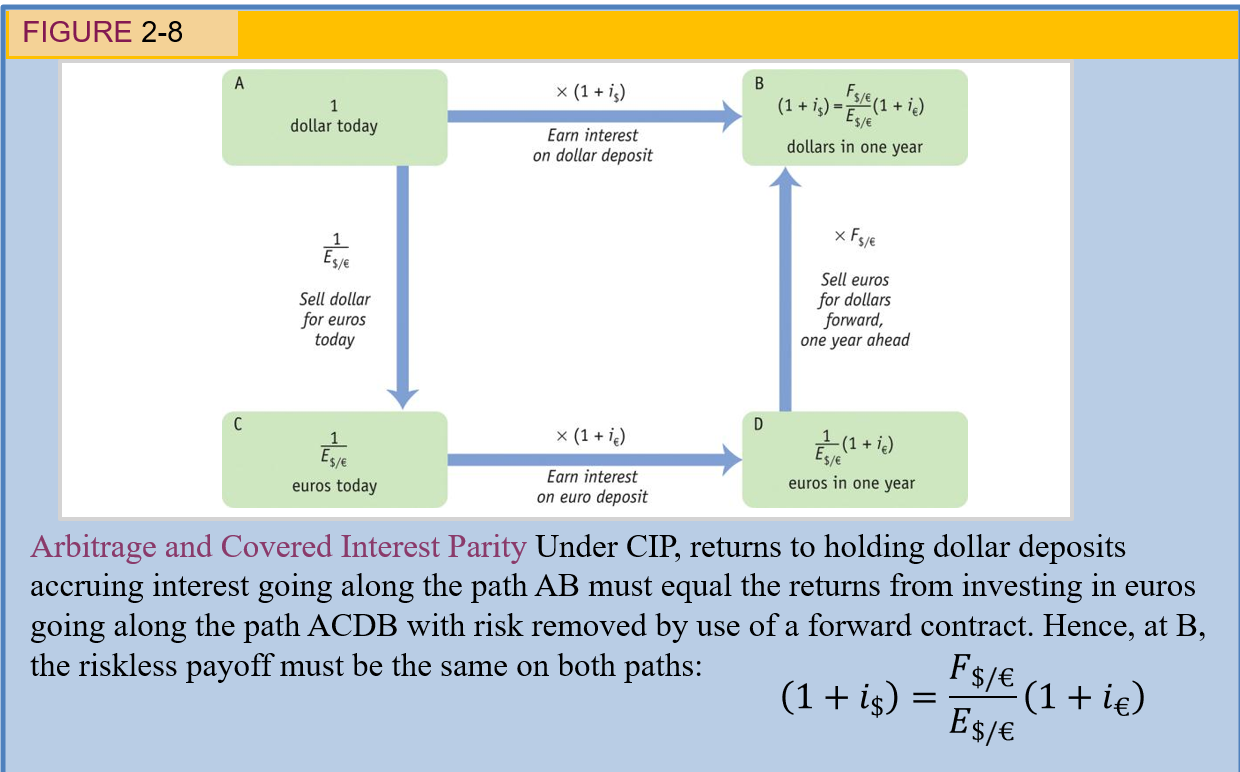
\includegraphics{pic1.png}
\end{frame}

\begin{frame}{CIP}
\phantomsection\label{cip-1}
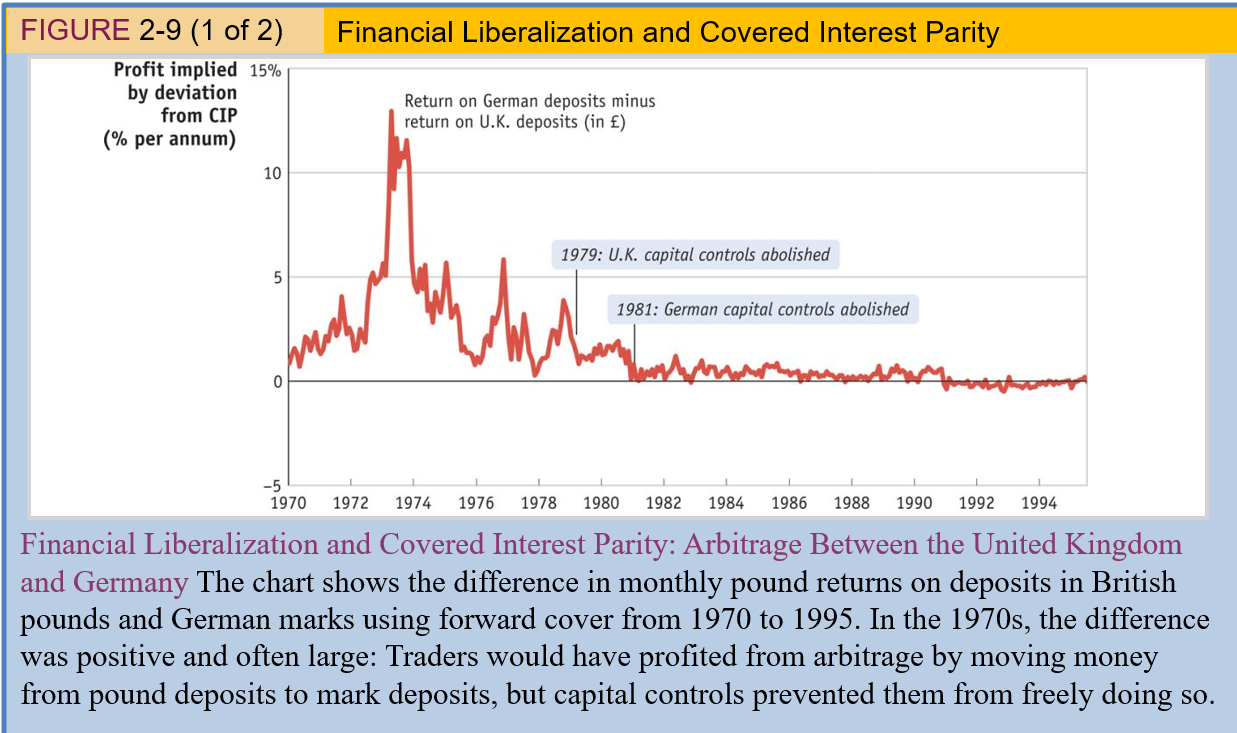
\includegraphics{pic2.png}
\end{frame}

\begin{frame}{Uncovered parity}
\phantomsection\label{uncovered-parity}
\begin{itemize}
\item
  Jika investor tidak membeli kontrak forward, maka ia harus menebak
  spot rate di tahun depan. Tebakan ini disebut juga \emph{expected
  exchange rate}, kita simbolkan \(E_{\$/€}^e\).
\item
  Jika kita tebak spot rate di tahun depan adalah \(E_{\$/€}^e\), maka
  kita akan mendapat \((1+i_{€})/E_{\$/€} \times E_{\$/€}^e\) dolar.
\end{itemize}

\[
\underbrace{(1+i_{\$})}_\text{Dollar return on dollar deposit}=\underbrace{(1+i_{€})\frac{E_{\$/€}^e}{E_{\$/€}}}_\text{Expected dollar return on euro deposit}
\]

\begin{itemize}
\tightlist
\item
  Ini disebut juga Uncovered Interest Parity (UIP)
\end{itemize}
\end{frame}

\begin{frame}{Determinan nilai tukar}
\phantomsection\label{determinan-nilai-tukar}
\begin{itemize}
\item
  UIP adalah sebuah kondisi no-arbitrase yang menjelaskan ekuilibrium di
  mana menabung di 2 mata uang berbeda memiliki nilai imbal balik yang
  sama, tanpa menggunakan kontrak forward.
\item
  Dengan IUP, kita dapat melihat determinan nilai tukar (spot rate) di
  mana:
\end{itemize}

\[
E_{\$/€}=E_{\$/€}^e \frac{1+i_{€}}{1+i_{\$}}
\]
\end{frame}

\begin{frame}{UIP}
\phantomsection\label{uip}
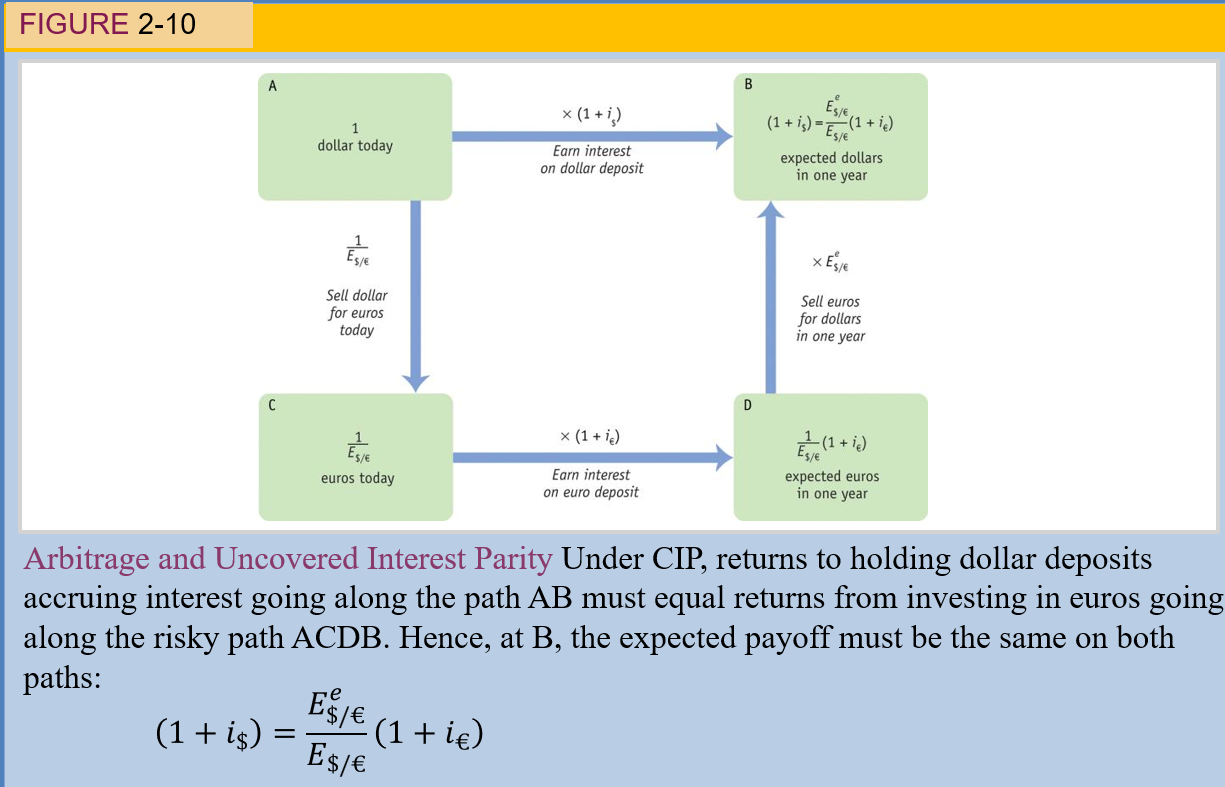
\includegraphics{pic3.png}
\end{frame}

\begin{frame}{Tentang aset}
\phantomsection\label{tentang-aset}
\begin{itemize}
\item
  Portolio seorang investor dapat terdiri dari saham, surat berharga,
  vila di Swiss, lukisan, deposito dan lain-lain dalam berbagai mata
  uang.
\item
  Atribut penting dari aset: return/imbal balik, risiko, dan likuiditas.
\item
  Return dari suatu aset adalah total pertumbuhan bersih dari
  portfolionya. Biasanya diukur tahunan.
\item
  Risiko aset maksudnya adalah volatilitas dari return aset tersebut.
\item
  likuiditas artinya seberapa mudah aset tersebut bisa dicairkan/dijual.
\item
  Hasil ramalan return kita katakan sebagai ekspektasi return.
\end{itemize}
\end{frame}

\begin{frame}{UIP dan CIP}
\phantomsection\label{uip-dan-cip}
\begin{itemize}
\tightlist
\item
  Jika kondisi UIP dan CIP terjaga. maka kita akan mendapati bahwa
\end{itemize}

\[
E_{\$/€}=F_{\$/€}
\]

\begin{itemize}
\item
  Meskipun nilai ekspektasi spot rate dan forward rate digunakan secara
  terpisah, tapi di ekuilibrium keduanya harusnya sama.
\item
  Akibatnya, bagi investor yang risk-neutral, risky dan riskless trade
  akan memberikan return yang sama.
\end{itemize}
\end{frame}

\begin{frame}{UIP dan CIP}
\phantomsection\label{uip-dan-cip-1}
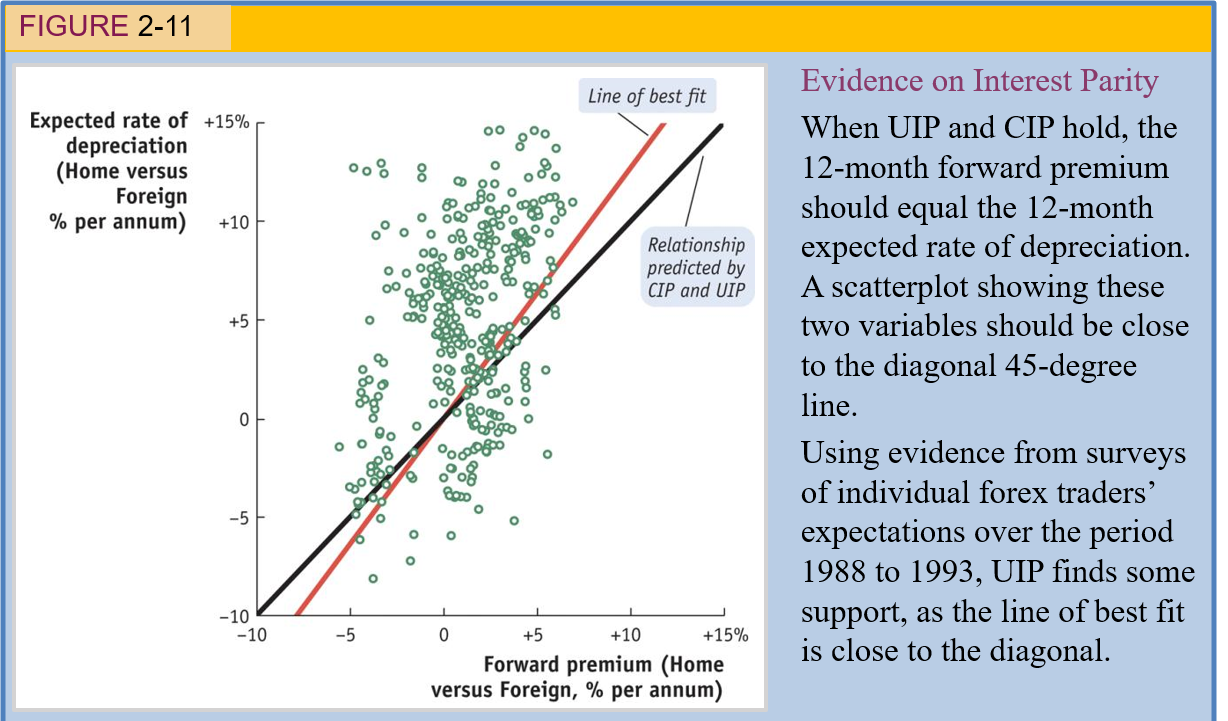
\includegraphics{pic4.png}
\end{frame}

\begin{frame}{UIP dan CIP}
\phantomsection\label{uip-dan-cip-2}
Aproksimasi dari UIP:

\[
i_\$=i_{€}+\frac{E_{\$/€}^e-E_{\$/€}}{E_{\$/€}}
\]

nilai ekspektasi biasanya sulit diukur, tapi jika UIP terjaga, maka kita
bisa menebak nilai ekspektasi berdasarkan rumus di atas.

Misalnya bunga dolar 4\% sementara euro di 3\%. Andai UIP terjaga, maka
ekspektasi depresiasi dolar tahun depan akan 1\%. Orang yang melakukan
arbitrase dari euro ke dolar akan dapat return yang sama dengan yang
nabung euro dari awal.
\end{frame}

\begin{frame}{UIP dan CIP}
\phantomsection\label{uip-dan-cip-3}
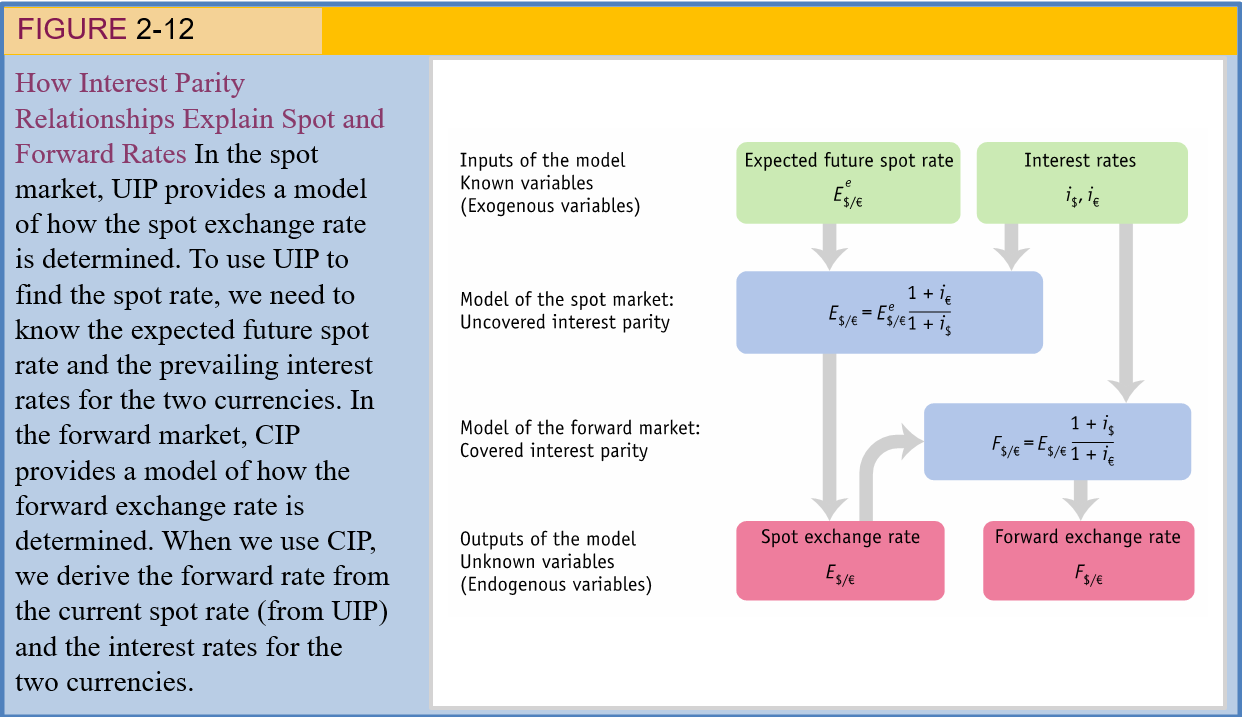
\includegraphics{pic5.png}
\end{frame}

\begin{frame}{Kesimpulan}
\phantomsection\label{kesimpulan}
\begin{itemize}
\item
  Nilai tukar mata uang suatu negara adalah harga dari mata uang
  tersebut dinilai dengan mata uang negara lain. Harga ini ditentukan di
  spot market pasar uang.
\item
  Nilai tukar Home naik berarti jumlah valas yang diperlukan untuk
  membeli mata uang Home semakin banyak, dan sebaliknya.
\item
  Nilai tukar digunakan untuk membandingkan harga barang dan jasa, serta
  aset keuangan dengan valas yang sama.
\item
  Ada banyak rezim nilai tukar, dari yang fixed sampai yang float.
\end{itemize}
\end{frame}

\begin{frame}{Kesimpulan}
\phantomsection\label{kesimpulan-1}
\begin{itemize}
\item
  Pasar uang didominasi oleh spot rate, dengan aktornya terutama bank
  komersil.
\item
  Pertukaran bebas nilai tukar mengakibatkan cross rate dan spot rate
  kurang lebih sama.
\item
  Riskless interest arbitrage mengakibatkan kondisi CIP, sementara risky
  interest arbitrage mengakibatkan kondisi UIP.
\item
  CIP menunjukkan determinan forward rate, sementara UIP menunjukkan
  determinan spot rate.
\end{itemize}
\end{frame}

\begin{frame}{Minggu depan}
\phantomsection\label{minggu-depan}
\begin{itemize}
\tightlist
\item
  kita akan melanjutkan pembahasan pergerakan nilai tukar jangka panjang
  dengan melibatkan harga-harga barang.
\end{itemize}
\end{frame}



\end{document}
